\section{Open-Source Orbit Propagators}
The development and adoption of open-source orbit propagators have transformed the field of astrodynamics, providing accessible, high-quality tools for a diverse range of applications. These propagators are pivotal for satellite trajectory prediction, mission analysis, and integrating advanced modeling techniques.

\subsection{Key Features and Comparisons}
Open-source orbit propagators vary in precision, supported orbital regimes, programming languages, and usability. Table~\ref{tab:propagators_sorted} summarizes the key features of popular tools:

\begin{itemize}
    \item \textbf{GMAT}: Excels in high-fidelity trajectory optimization for interplanetary and geostationary missions.
    \item \textbf{KASIOP}: Kinematic Analysis and Simulation of Orbits and Positions (KASIOP) serves as the demonstration platform for post-Newtonian perturbation modeling. %It integrates high-precision GNSS data and advanced relativistic corrections, providing a testbed for evaluating the impact of relativistic effects on satellite orbits.
    \item \textbf{Orekit}: A versatile library supporting GNSS, LEO, and interplanetary orbits with extensive customizability.
    \item \textbf{Skyfield}: A Python-based library focused on precise computations for orbital and astronomical ephemerides. %It provides an easy-to-use interface for tracking satellites, planets, and other celestial bodies, leveraging high-accuracy data from the IAU and JPL ephemerides. While its primary strength lies in astronomical tracking, Skyfield also supports TLE-based satellite propagation, making it a versatile tool for both astronomers and satellite engineers. Its Python implementation ensures accessibility for researchers and students.
    \item \textbf{NEOPROP}: Provides robust algorithms for near-Earth object tracking, incorporating advanced perturbation modeling.
    \item \textbf{Polyastro}: A Python-based library for rapid prototyping of astrodynamic applications, focusing on ease of use.
    \item \textbf{STK (Free Tier)}: Offers visualization and basic mission analysis capabilities, and prebuilt models suitable for educational and small-scale satellite projects.
    \item \textbf{Orbit Predictor}: Simplifies TLE-based propagation for Earth-orbiting objects, including CubeSats and the ISS.
\end{itemize}

%\begin{table}[htbp]
%\centering
%\caption{Comparison of Open-Source Orbit Propagators}
%\label{tab:propagators}
%\begin{tabular}{lccc}
%\hline
%\textbf{Tool} & \textbf{Precision} & \textbf{Special Features} & \textbf{Programming Language} \\
%\hline
%GMAT & High & Mission analysis, trajectory optimization & C++ \\
%Orekit & High & Highly customizable, GNSS support & Java \\
%NEOPROP & Moderate & NEO tracking, perturbation modeling & Proprietary \\
%Polyastro & Moderate & Rapid prototyping, visualization & Python \\
%Orbit Predictor & Basic & Simplified TLE propagation & Python \\
%\hline
%\end{tabular}
%\end{table}

\begin{landscape}
\begin{table}[htbp]
\centering
\begin{tabular}{lccc}
\textbf{Tool} & \textbf{Precision} & \textbf{Special Features} & \textbf{Programming Language} \\
\hline
GMAT & High & Mission analysis, trajectory optimization & C++ \\
KASIOP & High & Demonstration of PN corrections & Proprietary \\
Orekit & High & Customizable, GNSS, interplanetary support & Java \\
Skyfield & Moderate & Astronomical body tracking & Python \\
NEOPROP & Moderate & Perturbation modeling for NEOs & Proprietary \\
Polyastro & Moderate & Rapid prototyping, visualization & Python \\
STK (Free Tier) & Moderate & Visualization, GUI-based scenario analysis & Proprietary \\
Orbit Predictor & Basic & Simplified TLE propagation & Python \\
\end{tabular}
\caption{Comparison of Open-Source and Free Orbit Propagators (Sorted by Precision)}
\label{tab:propagators_sorted}
\end{table}
\end{landscape}

\subsection{Why Open Source Matters}
Open-source tools democratize access to advanced orbital mechanics, fostering collaboration, transparency, and innovation. They empower researchers, small satellite developers, and students to experiment without prohibitive costs.

\subsection{Emerging Trends}
The field of orbit propagation continues to evolve, with trends such as:
\begin{itemize}
    \item Integration of AI and machine learning to improve accuracy.
    \item Real-time data assimilation from GNSS and other sensors.
    \item Modular designs for extensibility and ease of use.
\end{itemize}

\subsection{Applications of Post-Newtonian Dynamics}
Post-Newtonian corrections are increasingly integrated into modern propagators, enhancing their capability to model relativistic effects essential for high-precision missions. Figure~\ref{fig:pn_corrections} illustrates these corrections and their relative impact.

\begin{figure}[htbp]
    \centering
    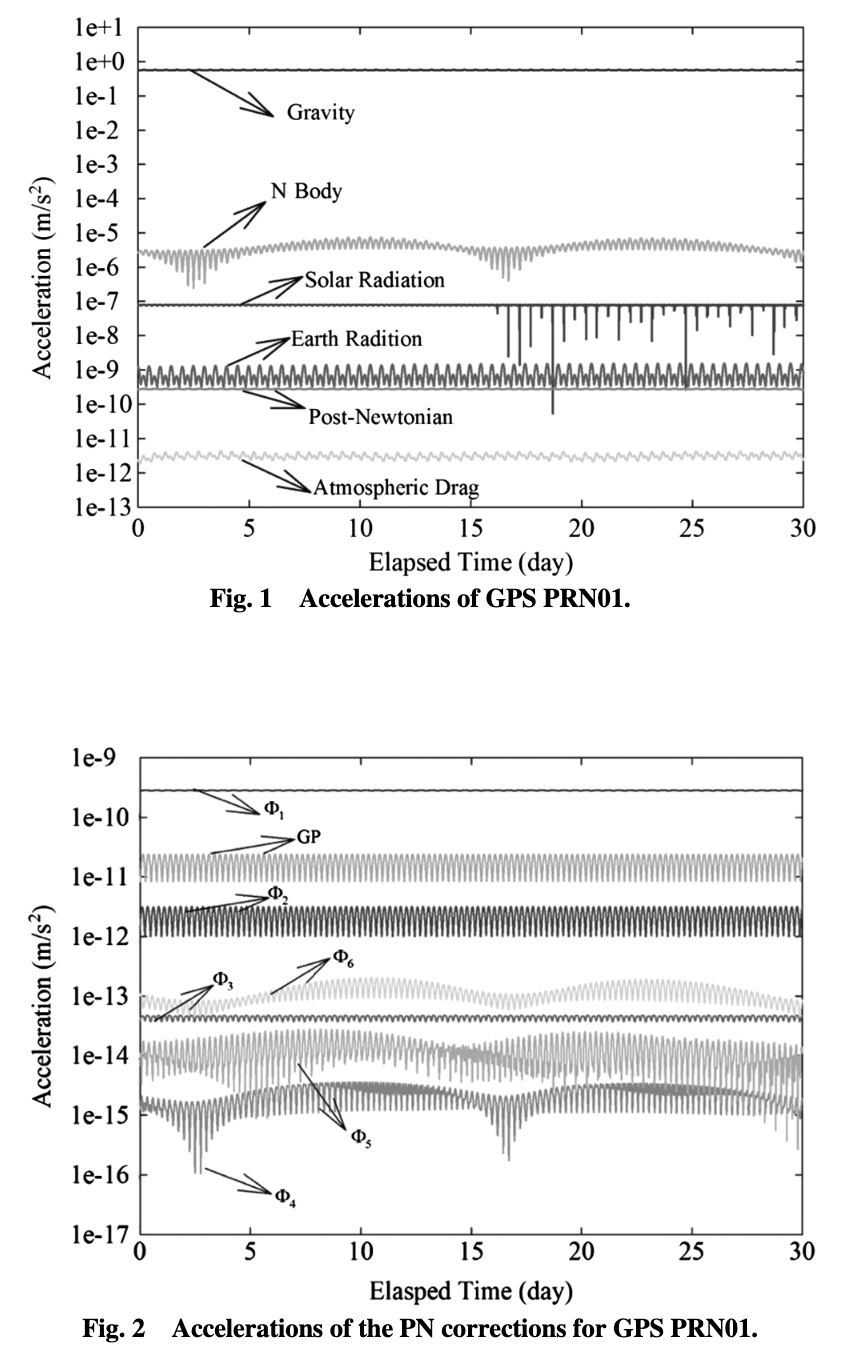
\includegraphics[ width = 4in ]{\pLocalGraphics/rho-fig.png}
    \caption{Accelerations of post-Newtonian corrections for GPS PRN01, highlighting the relative impact of various perturbations from \cite{roh2018numerical}. This work leverages KASIOP as a demonstration platform to evaluate the impact of post-Newtonian corrections on satellite dynamics.}
    \label{fig:pn_corrections}
\end{figure}

The dominant post-Newtonian corrections are
\begin{itemize}
    \item[\(\Phi_1\)] Schwarzschild perturbation: The largest contribution, caused by the spherically symmetric part of the Earth's geopotential.
    \item[\(\Phi_2\)] Lense–Thirring effect: A result of the Earth's constant rotation, also known as frame-dragging.
    \item[\(\Phi_3\)] Quadrupole relativistic effect: Due to the Earth's quadrupole moment, commonly associated with the \(J_2\) term.
    \item[\(\Phi_4\)] Nonlinear coupling of the Earth's monopole and solar gravitoelectric tidal field.
    \item[\(\Phi_5\)] Gravitomagnetic tidal perturbation: Related to the Earth's rotational effects.
    \item[\(\Phi_6\)] Gravitoelectric tidal perturbation: Due to external bodies in the solar system.
    \item[\(\Phi_7\)] Geodesic precession (de Sitter precession): A slow precession of the geocentric spatial frame relative to the barycentric frame.
\end{itemize}

\endinput  %  ==  ==  ==  ==  ==  ==  ==  ==  ==
